\chapter{Optimal Motion Planning for Humanoid Robots}
\label{chap:optimal-motion-planning}

The generation of the best possible trajectory that does not violate
any constraints imposed by the environment is an ubiquitous task in
both industrial and humanoid robotics. Numerous examples of successful
robotic applications in the domains of motion planning and optimal
control can be encountered in literature and industry. Very few
however, if none, consider the more general problem of optimal motion
planning for complex robots evolving in complex environments.

There are two established but still quite separate research areas that
both address a part of the optimal motion planning problem, namely
path planning and optimal control. This chapter aims at combining
state of the art developments of path planning and optimal control and
to create the algorithmic foundations to tackle optimal control
problems in cluttered environments. We thus propose a two-stage
framework for optimal motion planning on complex robots, where a
quasi-statically feasible path is first planned then optimized in
order to produce a dynamically feasible trajectory. We additionally
describe a simple method to automatically generate minimum bounding
capsules around exact robot body geometries represented by meshes; the
capsules are used to implement distance constraints for an optimal
control problem solver and achieve (self-)collision avoidance. The
whole framework is successfully applied to generate optimal
collision-free trajectories both in simulation and on the humanoid
robot HRP-2.

\section{Path Planning}

Sampling-based algorithms, such as Rapidly-exploring Random Trees
(RRT) which were presented in Section
\ref{subsec:chap1-sampling-algorithms}, are particularly powerful when
it comes to solving path planning problems in
high-dimension \cspace\thinspace and cluttered environments. In this
chapter, we rely on the same constrained RRT alogrithm that was
described in Chapter \ref{subsec:chap2-constraint-motion-planning} in
order to generate statically balanced paths on a submanifold
of \cspace.

Let us recall that an important feature of sampling-based algorithms
is their probabilistic completeness, i.e. their capacity to avoid
falling into local minima and to find a solution path if it
exists. They present however three drawbacks. First, due to their
sampling nature, the configuration \config{} might move in a random
fashion along the path $P$, which could lead to unnecessarily long and
unnatural paths. Second, we still need to apply a time parametrization
in order to transform the path into a trajectory. This is a
non-trivial task in the particular case of a humanoid robot, as we
must ensure its dynamic balance along the trajectory. Third, the
resulting paths are continuous but not $C^1$. The time-parametrized
motion thus needs to stop at each waypoint or to leave the planned
path around waypoints. Additional processing is thus needed to provide
a reshaped collision-free trajectory that can be executed on the
robot.

\section{Numerical Optimization}

Focus on jacobian-based optimal control

Following section largely based on Nocedal.

\subsection{Unconstrained Optimization}

$f:\mathbb R^n \rightarrow \mathbb R$

Problem:
\begin{equation}
\min_{\mathbf{x}}f(\mathbf{x}), \mathbf{x} \in \mathbb R^n
\end{equation}

Global minimizer:
\begin{equation}
f(\argmin{x}) \le f(\mathbf{x})~\forall \mathbf{x} \in \mathbb R^n
\end{equation}

local minimizer: $\exists$ a neighborhood $\mathcal{N}$ of
$\argmin{x}$ such that:
\begin{equation}
  f(\argmin{x} \le f(\mathbf{x})~\forall \mathbf{x} \in \mathcal{N}
\end{equation}

How to find a minimizer?

First-order nevessary conditions:
$\argmin{x}$ is a local minimizer, f continuously differentiable
($C^1$) in an open neighborhood of $\argmin{x} \Rightarrow
\nabla f(\argmin{x}) = \mathbf{0}$.

All points $\argmin{x}$ which satisfy $\nabla f(\argmin{x})$ are called
stationary points. Stationary points can correspond to minimizers,
maximizers, or saddle points of $f$. The second-order conditions are
then necessary to distinguish local minimizers:

$\argmin{x}$ is a local minimizer, f twice continuously differentiable
($C^2$) in an open neighborhood of $\argmin{x} \Rightarrow \nabla
f(\argmin{x}) = \mathbf{0}$ and $\nabla^2 f(\argmin{x})$ is positive
semi-definite (psd).

Note that if $F$ is convex and $C^1$, $\nabla f(x)$ is positive
definite (pd) $\forall~\mathbf{x}$, and it can be shown that anu
stationary point is a global minimizer.

One way of finding a minimizer of $f$ is to look for a stationary
point starting from an initial point $\arginit{x}$, and produce a
sequence of iterates $\{\mathbf{x}_k\}_{k=0}^{\infty}$ that terminates
when a termination condition is reached; this condition corresponds to
the point $\argmin{x}$ where no more progress can be made, up to a
specified tolerance $\epsilon > 0$.

Given an iterate $\mathbf{x_k}$, the next iterate $\mathbf{x_{k+1}}$
can be chosen based on information about f at $\mathbf{x_k}$ so that
$f(\mathbf{x_{k+1}})<f(\mathbf{x_k})$. There exist two main strategies
to do so:

\begin{enumerate}
\item Line search strategy: a direction $\mathbf{p_k}$ is first
  chosen, then a step length $\alpha_k > 0$ is computed such that it
  approximately solves the 1D minimization problem: $\min_{\alpha>0}
  f(\mathbf{x_k}+\alpha_k\mathbf{p}_k)$.
\item Trust region strategy: a local model $m_k$ of $f$ is
  constructed, and a direction $p_k$ is chosen inside a fixed-size
  trust region such that it approximately solves the minimization
  problem: $\min_{\mathbf{p_k}} m_k(\mathbf{x}_k+\mathbf{p}_k)$.
\end{enumerate}

Note that these two strategies are very similar as they try find
approximate solutions to simple optimization problems, which leads to
good performance. They mainly differ in the order in which the step
length and search direction are chosen. In the following section, we
will describe some of the most common line search strategies.

In what follows, $f_k$ denotes $f(\mathbf{x}_k)$ $\forall~k > 0$.

We introduce as an example the Rosenbrock function, or banana
function, defined as:

\begin{equation}
\mathbf{x} = (x,y) \in \mathbb R^2 r(\mathbf{x}) =
(1-x^2)+100(y-x^2)^2
\end{equation}

$r$ has only one minimizer $\argmin{x} = (1~1)$ and is commonly
used for benchmarking optimization algorithms.

\subsubsection{Steepest Descent Line Search}

Using a first-order Taylor approximation of $f$, it can be proved that:
\begin{equation}
\mathbf{p_k} = -\nabla f_k
\end{equation}
is the steepest descent direction, i.e. it is the direction along
which $f$ decreases locally around $\mathbf{x}_k$.

Add convergence rate:linear and explain.

Figure \ref{fig:chap3-unconstrained-steepest-descent} shows an example
of minimizing the Rosenbrock function. We show the first 20 iterates
when using a steepest descent line search and setting $\alpha_k$ to
1. The search direction $\mathbf{p_k}$ is always orthogonal to the
function contour line, as it is the direction that allows to decrease
$r$ quickly. Unfortunately, as the iterates reach the basin, keeping a
constant step size leads to a strong oscillation and convergence is
not achieved. This motivates the need for a good step size computation
method that will ensure a decrease of the function at each iteration.

\begin{figure}
  \centering
      {\def\svgwidth{0.5\linewidth}
        {\footnotesize
          \subimport*{src/chap3-optimal-motion-planning/figure/}
                     {unconstrained-steepest-descent.pdf_tex}
        }
      }
      \caption{Contour lines show the Rosenbrock function
        $r$. Starting from $\arginit{x}=(-0.6~-0.6)$, a steepest
        descent line search is used with a constant step size
        $\alpha_k=1$. The minimizer basin is reached very quickly,
        but large values of the step size then prevent minimizing the
        function. Note that the steepest descent direction is
        orthogonal to the contour lines of $r$.}
      \label{fig:chap3-unconstrained-steepest-descent}
\end{figure}

The Wolfe conditions offer the theoretical means and an easily
verifiable way to compute suitable step lengths. They are defined as:

\begin{equation}
\label{eq:chap3-wolfe-1}
f(\mathbf{x}_k + \alpha_k\mathbf{p}_k) \le
f(\mathbf{x_k}+c_1\alpha_k\nabla f_k^{\top}\mathbf{p_k}),
\end{equation}
\begin{equation}
\label{eq:chap3-wolfe-2}
\nabla f(\mathbf{x_k} + \alpha_k
\mathbf{p}_k)^{\top}\mathbf{p_k} \ge c_2 \nabla f_k^{\top}\mathbf{p_k},
\end{equation}

where $0 < c_1 < c_2 < 1$. Equation \ref{eq:chap3-wolfe-1} is called
the \emph{sufficient decrease} or \emph {Armijo condition}; it rejects
too small decreases in $f$. Equation \ref{eq:chap3-wolfe-2} is called
the \emph{curvature condition}, and it rejects too negative slopes
which might slow down convergence. In practice, $c_1$ is very small
and set to $10^{-4}$, while $c_2$ is set to a value ranging from $0.1$
to $0.9$.

The Wolfe conditions can be used to write a simple step length
computation algorithm, as described in Algorithm
\ref{alg:chap3-line-search-wolfe}. The idea is to start with a large
value of $\alpha_k$ and decrease it until the Wolfe conditions are
satisfied.

\begin{algorithm}
\caption{\texttt{StepLengthWolfe}($f$, $\mathbf{x}_k$, $\mathbf{p}_k$,
  $\alpha_k$, $\rho$, $it\_max$)}
\label{alg:chap3-line-search-wolfe}
\begin{algorithmic}
\STATE $it$ $\leftarrow$ $0$
\WHILE{Wolfe conditions are not verified \& $it < it\_max$}
\STATE {\color{red} // $\rho < 1$}
\STATE $\alpha_k$ $\leftarrow$ $\rho \alpha_k$ 
\STATE $it$ $\leftarrow$ $it + 1$
\ENDWHILE
\RETURN $\alpha_k$
\end{algorithmic}
\end{algorithm}

Figure \ref{fig:chap3-unconstrained-steepest-descent-wolfe} shows the
solution to the same problem as in Figure
\ref{fig:chap3-unconstrained-steepest-descent} with the Wolfe
conditions enforced at each iteration. The minimizer
$\argmin{x}=(1~1)$ is reached after around 5000 iterations. Such a
high number is mainly due to the zigzagging behavior which prevents
quickly reaching the minimizer, as shown in Figure
\ref{fig:chap3-unconstrained-steepest-descent-wolfe-b}.

\begin{figure}
  \centering
  \begin{subfigure}{0.4\columnwidth}
    \centering
        {\def\svgwidth{\linewidth}
          {\footnotesize
            \subimport*{src/chap3-optimal-motion-planning/figure/}
                       {unconstrained-steepest-descent-wolfe.pdf_tex}
          }
        }
        \caption{FIXME}
        \label{fig:chap3-unconstrained-steepest-descent-wolfe-a}
  \end{subfigure}
  \begin{subfigure}{0.4\columnwidth}
    \centering
        {\def\svgwidth{\linewidth}
          {\footnotesize
            \subimport*{src/chap3-optimal-motion-planning/figure/}
                       {unconstrained-steepest-descent-wolfe-zoom.pdf_tex}
          }
        }
        \caption{FIXME}
        \label{fig:chap3-unconstrained-steepest-descent-wolfe-b}
  \end{subfigure}
  \caption{FIXME}
  \label{fig:chap3-unconstrained-steepest-descent-wolfe}
\end{figure}

\subsubsection{Newton Line Search}

Assuming that $f$ is $C^2$ and using a second-order Taylor
approximation at $\mathbf{x}_k$, we can derive the Newton direction:
\begin{equation}
\mathbf{p_k} = -\nabla^2 f_k^{-1} \nabla f_k;
\end{equation}
$\mathbf{x}_{k+1}=\mathbf{x_k}+\mathbf{p_k}$ is then the minimizer of
the local quadratic approximation of $f$. The Newton direction has a
natural step length $\alpha_k=1$. Nevertheless the Wolfe conditions
still need to be verified to make sure that there is an actual
decrease of the exact function $f$. Figure
\ref{fig:chap3-unconstrained-newton-wolfe} shows the sequence of
iterates when applying a Newton line search to find the minimizer of
the Rosenbrock function. It is clear in Figure
\ref{fig:chap3-unconstrained-newton-wolfe-quad} how the next iterate
is the minimizer of the local quadratic approximation of the objective
function.

\begin{figure}
  \centering
  \begin{subfigure}{0.4\columnwidth}
    \centering
        {\def\svgwidth{\linewidth}
          {\footnotesize
            \subimport*{src/chap3-optimal-motion-planning/figure/}
                       {unconstrained-newton-wolfe.pdf_tex}
          }
        }
        \caption{FIXME}
        \label{fig:chap3-unconstrained-newton-wolfe-a}
  \end{subfigure}
  \begin{subfigure}{0.4\columnwidth}
    \centering
        {\def\svgwidth{\linewidth}
          {\footnotesize
            \subimport*{src/chap3-optimal-motion-planning/figure/}
                       {unconstrained-newton-wolfe-quad.pdf_tex}
          }
        }
        \caption{FIXME}
        \label{fig:chap3-unconstrained-newton-wolfe-quad}
  \end{subfigure}
  \caption{FIXME}
  \label{fig:chap3-unconstrained-newton-wolfe}
\end{figure}

The Newton line search is very efficient and exhibits quadratic
convergence. However, besides knowing how to compute the Jacobian of
$f$, we need to know how to compute the Hessian of $f$ and this is not
always a trivial task.

\subsubsection{Quasi-Newton Line Search}
\label{subsubsec:chap3-quasi-newton-line-search}

Instead of relying on the Hessian, a quasi-Newton line search relies
on using an approximation of $\nabla^2 f$ when it is not possible to
compute it. The search direction is then given by:
\begin{equation}
p_k=-\mathbf{B}_k^{-1}\nabla f_k,
\end{equation}
where $\mathbf{B}_k\approx\nabla^2 f$ is a symmetric nonsingular
matrix.

Several algorithms for deriving approximates $\mathbf{B_k}$ exist, the
best one being the Broyden-Fletcher-Goldfarb-Shanno (BFGS) method, as
described in Algorithm \ref{alg:chap3-bfgs}. It relies on updating the
$\mathbf{H}_k = \mathbf{B}_k^{-1}$ while the iterative optimization is
taking place. As an initial value $\mathbf{H}_0=\mathbf{I}$ is given,
the line search behaves like a steepest descent line search for the
first iterations, converging towards a Newton line search as the
optimization advances and as the approximation is closer to the real
Hessian. The BFGS line search exhibits then super linear convergence.

limited memory version for large-squcale problems.

\begin{algorithm}
\caption{\texttt{BFGS}($\arginit{x}$, $\epsilon$)}
\label{alg:chap3-bfgs}
\begin{algorithmic}
\STATE $\mathbf{H}_0$ $\leftarrow$ $\mathbf{I}$, $k$ $\leftarrow$ $0$
\WHILE{$||\nabla f_k|| > \epsilon$}
\STATE {\color{red} // Search direction}
\STATE $\mathbf{p}_k$ $\leftarrow$ $-\mathbf{H}_k\nabla f_k$
\STATE {\color{red} // Line search with Wolfe conditions}
\STATE $\mathbf{x}_{k+1}$ $\leftarrow$ $\mathbf{x}_k + \alpha_k\mathbf{p}_k$
\STATE $\mathbf{s}_k$ $\leftarrow$ $\mathbf{x}_{k+1} - \mathbf{x}_k$
\STATE $\mathbf{y}_k$ $\leftarrow$ $\nabla f_{k+1} - \nabla f_k$
\STATE $\rho_k$ $\leftarrow$ $\frac{1}{\mathbf{y}_k^{\top}\mathbf{s}_k}$
\STATE {\color{red} // BFGS update of the Hessian inverse}
\STATE $\mathbf{H}_{k+1}$ $\leftarrow$ $(\mathbf{I}-\rho_k\mathbf{s}_k\mathbf{y}_k^{\top})\mathbf{H}_k(\mathbf{I}-\rho_k\mathbf{y}_k\mathbf{s}_k^{\top})+\rho_k\mathbf{s}_k\mathbf{s}_k^{\top}$
\STATE $k$ $\leftarrow$ $k + 1$
\ENDWHILE
\end{algorithmic}
\end{algorithm}

\begin{figure}
  \centering
      {\def\svgwidth{0.5\linewidth}
        {\footnotesize
          \subimport*{src/chap3-optimal-motion-planning/figure/}
                     {unconstrained-quasi-newton-wolfe.pdf_tex}
        }
      }
      \caption{FIXME}
      \label{fig:chap3-unconstrained-quasi-newton-wolfe}
\end{figure}

FIXME commenter figure.

\subsection{Constrained Optimization}

\begin{equation}
\label{eq:chap3-nlp}
\min_{\mathbf{x} \in \mathbb R^n}
f(\mathbf{x}),\text{ such that }
\left\{\begin{array}{cc}
c_i(\mathbf{x}) = 0, & i \in \mathcal{E} \\%
c_i(\mathbf{x}) \ge 0, & i \in \mathcal{I} %
\end{array}\right.
\end{equation}

The gradient of f should lie in the subspace spanned by the constraint
gradients

Gradient of f and constraint colinear. In general case, gradient f can
be written as a linear combination of active constraints gradients. The
components of gradient f in this basis are called the \emph{Lagrange
  multipliers}.

\emph{Lagrangian}:
\begin{equation}
\mathcal{L}(\mathbf{x},\boldsymbol{\lambda}) =
f(\mathbf{x})-\sum_{i\in\mathcal{E}\cup\mathcal{I}}
\lambda_ic_i(\mathcal{x})
\end{equation}

\emph{Active set} at a feasible point $\mathbf{x}$:
\begin{equation}
\mathbf{A}(\mathbf{x})=\mathcal{E}\cup{i \in \mathcal{I}:
  c_i(\mathbf{x})=0}
\end{equation}

The Karush-Kuhn-Tucker (KKT) first-order necessary conditions:
\begin{equation}
\label{eq:chap3-kkt}
\begin{array}{crcl}
a) & \nabla_{\mathbf{x}}\mathcal{L}(\argmin{x}, \boldsymbol{\lambda}^\star) & = & \mathbf{0} \\%
b) & c_i(\argmin{x}) & = & 0 \qquad \forall i \in \mathcal{E} \\%
c) & c_i(\argmin{x}) & \ge & 0 \qquad \forall i \in \mathcal{I}\\%
d) & \lambda_i^{\star} & \ge & 0 \qquad \forall i \in \mathcal{I}\\%
e) & \lambda_i^{\star} c_i(\argmin{x}) & = & 0 \qquad \forall i \in \mathcal{E}\cup\mathcal{I}%
\end{array}
\end{equation}

$f(\argmin{x}) = \mathcal{L}(\argmin{x}, \boldsymbol{\lambda}^\star)$ because of
the complementarity condition $e)$ in Equation \ref{eq:chap3-kkt}.

\subsection{Quadratic Programming}

\emph{Quadratic program (QP)}: quadratic objective function, linear
constraints.

\begin{equation}
\label{eq:chap3-qp}
\min_{\mathbf{x} \in \mathbb R^n}
q(\mathbf{x})=\frac{1}{2}\mathbf{x}^{\top}\mathbf{G}\mathbf{x}
+\mathbf{c}^{\top}\mathbf{x},\text{ such that }
\left\{\begin{array}{cc}
\mathbf{a}_i^{\top}\mathbf{x} = b_i, & i \in \mathcal{E} \\%
\mathbf{a}_i^{\top}\mathbf{x} \ge b_i, & i \in \mathcal{I} %
\end{array}\right. ~\mathbf{G}\text{ symmetric.}
\end{equation}

Convex QP $\Leftrightarrow$ $\mathbf{G}$ psd. Local minimizer is also
global minimizer.

Non-convex QP $\Leftrightarrow$ $\mathbf{G}$ not psd. Possibly several
solutions.

\subsubsection{Equality-constrained QP}

\begin{equation}
\label{eq:chap3-qp-eq}
\min_{\mathbf{x} \in \mathbb R^n}
q(\mathbf{x})=\frac{1}{2}\mathbf{x}^{\top}\mathbf{G}\mathbf{x}
+\mathbf{c}^{\top}\mathbf{x},\text{ such that }
\mathbf{A}\mathbf{x} = b
\qquad \mathbf{A} \text{ full rank.}
\end{equation}

The KKT conditions given in Equation \ref{eq:chap3-kkt} imply that the
solution $\argmin{x}$ verifies:

\begin{equation}
  \label{eq:chap3-qp-kkt}
  \left(\begin{matrix}
    \mathbf{G} & -\mathbf{A}^{\top} \\
    \mathbf{A} & \mathbf{0}
  \end{matrix}\right)
  \left(\begin{matrix}
    \argmin{x} \\
    \boldsymbol{\lambda}^{\star}
  \end{matrix}\right)
  = \left(\begin{matrix}
    -\mathbf{c} \\
    \mathbf{b}
  \end{matrix}\right)  
  \overset{\argmin{x}=\mathbf{x}+\mathbf{p}}\Longleftrightarrow
  \left(\begin{matrix}
    \mathbf{G} & \mathbf{A}^{\top} \\
    \mathbf{A} & \mathbf{0} \\
  \end{matrix}\right)
  \left(\begin{matrix}
    -\mathbf{p} \\
    \boldsymbol{\lambda}^{\star}
  \end{matrix}\right)
  = \left(\begin{matrix}
    \mathbf{g} \\
    \mathbf{h}
  \end{matrix}\right)
  \quad
  \left\{\begin{matrix}
      \mathbf{h} = \mathbf{A}\mathbf{x} - \mathbf{b} \\
      \mathbf{g} = \mathbf{c} + \mathbf{G}\mathbf{x} \\
      \mathbf{p} = \argmin{x} - \mathbf{x}
    \end{matrix}\right.
\end{equation}

The final linear system in Equation \ref{eq:chap3-qp-kkt} is called
the \emph{KKT system}. It can be solved using standard linear algebra
techniques, and its solution gives the update $\mathbf{p}$ which leads
directly to the minimizer $\argmin{x}$ of $q$.

\begin{figure}
  \centering {\def\svgwidth{0.5\linewidth} {\footnotesize
      \subimport*{src/chap3-optimal-motion-planning/figure/}
                 {qp-equality.pdf_tex} } }
      \caption{FIXME}
      \label{fig:chap3-qp-equality}
\end{figure}

show in figure solution for same quadratic function and different
equality constraints.

The associated Lagrange multiplier is higher as the constrained
minimizer is further from the unconstrained minimum. Intuitively, we
can see Lagrange multiplier give an idea of the ``force'' which the
constraints are exerting on the constrained minimizer.

\subsubsection{Inequality-Constrained QP}

Solve the general system presented in Equation \ref{eq:chap3-qp}.

Several types of method such as active-set, gradient-projection and
interior-point. We describe here the active-set method for solving
inequality-constrained QP.

\begin{algorithm}
\caption{\texttt{ActiveSetSolve}($\arginit{x}$)}
\label{alg:chap3-active-set}
\begin{algorithmic}
\STATE {\color{red} // Initialize active set}
\STATE $\mathcal{W}_0$ $\leftarrow$ subset of the active constraints at $\arginit{x}$
\FOR{$k=0,1,2,...$}
\STATE {\color{red} // Find minimizer of equality-constrained QP using active constraints}
\STATE $(\mathbf{p_k}~\boldsymbol{\lambda}_{k+1})$ $\leftarrow$ \texttt{SolveKKTSystem}($\mathbf{W_k}$)
\IF{$\mathbf{p}_k=\mathbf{0}$}
\IF{$\lambda_{k+1,i} \ge 0~\forall i \in \mathcal{W}_k\cap\mathcal{I}$}
\STATE {\color{red} // All inequality constraints in the active set are active}
\RETURN ($\mathbf{x}_k,\boldsymbol{\lambda}_{k+1)}$
\ELSE
\STATE {\color{red} // At least one inequality constraint in the active set is inactive}
\STATE {\color{red} // Remove the one that is ``least active''}
\STATE $\mathcal{W}_{k+1}$ $\leftarrow$ $\mathcal{W}_k \backslash \{\text{arg}\min_{j\in\mathcal{W}_k\cap\mathcal{I}}\lambda_{k+1,j}\}$
\ENDIF
\ELSE
\STATE {\color{red} // Compute $\alpha_k$ such that the constraints which are \emph{not} in the active set are not violated}
\STATE $\alpha_k$ $\leftarrow$ $\min_{\substack{i\notin\mathcal{W}_k\\\mathbf{a}_i^{\top}\mathbf{p}_k<0}} \frac{b_i-\mathbf{a}_i^{\top}\mathbf{x}_k}{\mathbf{a}_i^{\top}\mathbf{p}_k}$
\STATE $\mathbf{x}_{k+1}$ $\leftarrow$ $\alpha_k\mathbf{p}_k$
\IF{$\alpha_k<1$}
\STATE {\color{red} // At least one constraint which is not the active set is active, add one}
\STATE $\mathcal{W}_{k+1}$ $\leftarrow$ $\mathcal{W}_k\cup\{$one blocking constraint$\}$
\ELSE
\STATE {\color{red} // Keep the same active set}
\STATE $\mathcal{W}_{k+1}$ $\leftarrow$ $\mathcal{W}_k$
\ENDIF
\ENDIF
\ENDFOR
\end{algorithmic}
\end{algorithm}

\begin{figure}
  \centering
      {\def\svgwidth{0.5\linewidth}
        {\footnotesize
          \subimport*{src/chap3-optimal-motion-planning/figure/}
                     {qp-inequality.pdf_tex}
        }
      }
      \caption{FIXME}
      \label{fig:chap3-qp-inequality}
\end{figure}

Figure \ref{fig:chap3-qp-inequality} shows the minimization of a
quadratic objective function with one linear equality constraint and
two linear inequality constraints. Minimizer is found with the
previously described active-set method.

\subsection{Nonlinear Programming}

\emph{Non-linear program (NLP)}: solve the general problem presented
in Equation \ref{eq:chap3-nlp}.

\subsubsection{Sequential Quadratic Programming}

\emph{Sequential Quadratic Program (SQP)}

Build local quadratic approximation of the objective function and
linearized approximation of the constraints in order to obtain a
\emph{QP subproblem}:

\begin{equation}
\min_{\mathbf{p}}\frac{1}{2}\mathbf{p}_k^{\top}\nabla_{\mathbf{x}\mathbf{x}}^2\mathcal{L}(\mathbf{x}_k,\boldsymbol{\lambda}_k)\mathbf{p}+\nabla f(\mathbf{x}_k)^{\top}\mathbf{p}+f(\mathbf{x}_k)
\text{ s.t. }
\left\{\begin{array}{cc}
\nabla c_i(\mathbf{x}_k)^{\top}+c_i(\mathbf{x}_k) = 0, & i \in \mathcal{E} \\
\nabla c_i(\mathbf{x}_k)^{\top}+c_i(\mathbf{x}_k) \ge 0, & i \in \mathcal{I}
\end{array}\right.
\end{equation}

Solve the QP subproblem, with active-set methods for instance, and
repeat iteratively until the convergence test is satisfied.

\begin{algorithm}
\caption{\texttt{SQPSolve}($\arginit{x}$,$\boldsymbol{\lambda}_0$, $\epsilon$)}
\label{alg:chap3-sqp}
\begin{algorithmic}
\FOR{$k=0,1,2,...$}
\STATE Evaluate $f_k$, $\nabla f_k$, $c_i(\mathbf{x}_k)$, $\nabla c_i(\mathbf{x}_k)$, $\nabla_{\mathbf{x}\mathbf{x}}^2\mathcal{L}(\mathbf{x}_k,\boldsymbol{\lambda}_k)$
\STATE $(\mathbf{p}_k, \boldsymbol{\lambda}_{k+1})$ $\leftarrow$ \texttt{ActiveSetSolve}($\mathbf{x}_k$)
\STATE $\mathbf{x}_{k+1}$ $\leftarrow$ $\mathbf{x}_k + \alpha_k\mathbf{p}_k$
\IF{convergence test satisfied for tolerance $\epsilon$}
\RETURN $(\mathbf{x}_{k+1},\boldsymbol{\lambda}_{k+1})$
\ENDIF
\ENDFOR
\end{algorithmic}
\end{algorithm}

Requires us to derive the Hessian of objective function and
constraints. Solution: use BFGS as in Section
\ref{subsubsec:chap3-quasi-newton-line-search}.

merit function: sufficient decrease of function and sufficient
feasibility with respect to equality and inequality constraints.

example: $l_1$ merit function

\begin{figure}
  \centering
      {\def\svgwidth{0.5\linewidth}
        {\footnotesize
          \subimport*{src/chap3-optimal-motion-planning/figure/}
                     {sqp.pdf_tex}
        }
      }
      \caption{FIXME}
      \label{fig:chap3-sqp}
\end{figure}

Iterates can be infeasible. Only final solution is guaranteed to be
feasible.

\subsubsection{Interior-Point Methods for Nonlinear Programming}

We introduce briefly \emph{interior-point methods}, also known as
\emph{log-barrier methods}. They propose an alternative to SQP and are
also very powerful when used to solve large-scale NLP.

Their principle is the following: a slack variable $\mathbf{s}$ is
introduced to reformulate the general NLP as:

\begin{equation}
\label{eq:chap3-nlp-slack}
\min_{\mathbf{x} \in \mathbb R^n}
f(\mathbf{x}),\text{ such that }
\left\{\begin{array}{cc}
c_i(\mathbf{x}) = 0, & i \in \mathcal{E} \\%
c_i(\mathbf{x})-s_i = 0, & i \in \mathcal{I} \\%
s_i \ge 0, & i \in \mathcal{I} %
\end{array}\right.
\end{equation}

A parameter $\mu>0$ is also introduced, which allows us to obtain the
\emph{perturbed KKT conditions}:

\begin{equation}
\label{eq:chap3-kkt-perturbed}
\begin{array}{crcl}
a) & \nabla f(\mathbf{x}) - \mathbf{A}_\mathcal{E}^{\top}(\mathbf{x})\mathbf{y} - \mathbf{A}_\mathcal{I}^{\top}(\mathbf{x})\mathbf{z} & = & \mathbf{0} \\%
b) & \mathbf{c}_{\mathcal{E}}(\mathbf{x}) & = & \mathbf{0} \\%
b')& \mathbf{c}_{\mathcal{I}}(\mathbf{x}) - \mathbf{s}& = & \mathbf{0} \\%
c) & \mathbf{s} & \succeq & \mathbf{0} \\%
d) & \mathbf{z} & \succeq & \mathbf{0} \\%
e) & \mathbf{S}\mathbf{z} & = & \mu\mathbf{e}, \\%
\end{array}
\end{equation}

with $\mathbf{c}_{\mathcal{E}}$, $\mathbf{c}_{\mathcal{I}}$ denoting
the constraints vector, $\mathbf{A}_\mathcal{E}(\mathbf{x})$,
$\mathbf{A}_\mathcal{I}(\mathbf{x})$ denoting their respective
Jacobians, $\mathbf{y}$, $\mathbf{z}$ denoting the Lagrange
multipliers, $\mathbf{S}=\text{diag}(s_i)$ and
$\mathbf{e}^\top=\left(\begin{matrix}1&\cdots&1\end{matrix}\right)$.

The variables $\mathbf{s}$ and $\mathbf{z}$ are eliminated from the
KKT conditions:

\begin{equation}
\forall i \in \mathcal{I}
\left.\begin{array}{r}
s_iz_i - \mu = 0\\
c_i(\mathbf{x})-s_i = 0
\end{array}\right\}
\Rightarrow
z_i=\frac{\mu}{c_i(\mathbf{x})},
\end{equation}

and substituted in
$\nabla_{\mathbf{x}}\mathcal{L}(\mathbf{x},\mathbf{y},\mathbf{z})$
in Equation \ref{eq:chap3-kkt-perturbed}$a)$:

\begin{equation}
\begin{array}{c}
\nabla f(\mathbf{x}) - \mathbf{A}_{\mathcal{E}}^{\top}(\mathbf{x}) -
\sum_{i\in\mathcal{I}}\frac{\mu}{c_i(\mathbf{x})}\nabla
c_i(\mathbf{x})=\mathbf{0} \\
\Updownarrow \\
\min_{\mathbf{x}}P(\mathbf{x};\mu)=f(\mathbf{x}) -
\mu\sum_{i\in\mathcal{I}}\text{log}c_i(\mathbf{x}) \quad\text{
  such that }\mathbf{c_{\mathcal{E}}=\mathbf{0}}
\end{array}
\end{equation}

Finding the stationary points of the Lagrangian of the original
problem is then equivalent to minimizing the equality-constrained
\emph{log-barrier function} $P(\mathbf{x};\mu)$ and making $\mu
\rightarrow 0$.

Write algorithm? inner loop: quadratic approximations to find
$\mathbf{x}^\star(\mu)$, outer loop: decrease $\mu$. Confirm with
Nicolas.

move along central path $\{\mathbf{x}^\star(\mu)\}_k$: solution always
feasible

\subsubsection{Conclusion}

SQP and IP methods equally efficient for solving large-scale NLP
problems.

SQP: a large number of inexpensive steps (small linear systems with
only active constraints, but active-search method runs a lot of
times), intermediate iterates might not be feasible. Easy to
warm-start

IP: a small number of expensive steps (larger linear system), iterates
all feasible. Harder to warm-start.

\section{Optimal Control}

Given a dynamic model, let:
\begin{itemize}
\item $t$ denotes the time variable,
\item \state{} denotes the state vector,
\item \control{} denotes the control vector,
\item $T$ denotes the trajectory duration,
\item $L$ denotes the Lagrangian term (also cost rate) of the
  objective function,
\item $\Phi$ denotes the Mayer term (also terminal cost?) of the
  objective function,
\item \dfcn{} denotes the \emph{ordinary differential equation (ODE)}
  of the model,
\item \eqcstr{} denotes the equality constraint vector function,
\item \ineqcstr{} denotes the inequality constraint vector function,
\item \bndcstr{} denotes the boundary conditions vector function.
\end{itemize}

An optimal control problem can be written as follows:

\label{OCP}
\begin{equation}
  \min_{\mathbf{x} (\cdot), \mathbf{u} (\cdot), T} \ \ 
  J(\mathbf{x}(t),\mathbf{u}(T),T) = \int_{0}^{T}L (\mathbf{x}(t), \mathbf{u}(t))dt + \Phi(\mathbf{x}(T))
  \label{OCP:Obj}
\end{equation}
\ \ \ subject to:

\begin{equation}
  \begin{array}{rcl}
  \dot{\mathbf{x}} (t) & = & \mathbf{f}(t, \mathbf{x}(t), \mathbf{u}(t))
  \label{OCP:Model}
  \\
  \mathbf{g}(t, \mathbf{x}(t), \mathbf{u}(t)) & = & \mathbf{0},
  \\
  \mathbf{h}(t, \mathbf{x}(t), \mathbf{u}(t)) & \succeq & \mathbf{0}%,
  \\
  \mathbf{r} (\mathbf{x}(0), \mathbf{x}(T)) & = & \mathbf{0}.
  \\
  \end{array}
\end{equation} 

FIXME: add interval [0,T] next to constraint validity (with explanation?)

\begin{figure}
  \centering
      {\def\svgwidth{0.9\linewidth}
        \subimport*{src/chap3-optimal-motion-planning/figure/}
                   {optimal-control-problem.pdf_tex}
      }
      \caption{Optimal control problem}
      \label{fig:chap3-optimal-control-problem}
\end{figure}

\subsection{Hamilton-Jacobi-Bellman Equation}

continuous extension of dynamic programming.

Richard Bellman's \emph{Optimality principle}

Optimal control for the unconstrained case

\emph{Hamilton Jacobi Bellman (HJB) partial differential equation}:

$v = J(\mathbf{x}(t),\mathbf{u}(t),T)$

\begin{equation}
\label{eq:chap3-hjb}
\dot{v} + \min_{\mathbf{x} (\cdot), \mathbf{u} (\cdot),
  T}(\nabla_{\mathbf{x}} v^{\top}f(t, \mathbf{x}(t), \mathbf{u}(t)) +
L (\mathbf{x}(t), \mathbf{u}(t)) = 0
\end{equation}

$v$ is also called the value function.

Equation \ref{eq:chap3-hjb} can be solved backwards in time, just as
in discrete-time dynamic programming, starting from $t=T$ and ending
at $ t=0$.

curse of dimensionality (cf todorov).

\subsection{Indirect Methods,Pontryagin}

\emph{Maximum (or Minimum) principle}

Minimize the \emph{Hamiltonion} $\mathcal{H}$ defined as:

\begin{equation}
\mathcal{H}(\mathbf{x}(t),\mathbf{u}(t),T) = \nabla_{\mathbf{x}}
v^{\top}f(t, \mathbf{x}(t), \mathbf{u}(t)) + L (\mathbf{x}(t),
\mathbf{u}(t))
\end{equation}

continuous extension to Lagrange multipliers.

define hamiltonian as objective function defined in HJB equation.

remarkable: Turn PDE to ODE by defining costate variable as
$\nabla_{\mathbf{x}} v$.

Solve Boundary Value Problem: very easy especially when controls
appear linearly in dynamics and quadratically in cost rate.

complexity linear with state dimension.

How to handle constrained case?

\subsection{Direct Methods}

Also known as “First discretize, then optimize” methods.

infinite-dimensional variables => discretization of controls: reduction to a finite
dimension variables

transcribe infinite problem into finite dimensional NLP.

Pros:
Can use state-of-the-art methods for NLP solution.
Can treat inequality constraints and multipoint constraints much
easier.

Cons:
suboptimal/approximate solution but still ok if chosen properly.

Nowadays most commonly used methods due to their easy
applicability and robustness.

FIXME: state (and not control) parametrization: where does it fall?:
not collocation, not single-shooting, not
multiple-shooting. Trajectory is C2 by design, no need to add
additional constraints as in multiple shooting. works for problems
where the final solution (such as the input controls) can be easily
derived from the state. \cite{sirinesa1981}

Add figures in inkscape? or as Martin?

\subsubsection{Direct Single-Shooting}

\cite{hicks1971approximation,sargent1978development}

Discretize controls $\mathbf{u}(t)$ on a fixed grid
$0=t_0<t_1<\ldots<t_N=T$. States $\mathbf{x}(t)$ are regarder as
dependent variables on $[0,T]$; numerical integration is used in order
to obtain state as function $\mathbf{x}(t,\mathbf{q})$ of finitely
many control parameters
$\mathbf{q}=(\mathbf{q}_0,\mathbf{q}_1,\ldots,\mathbf{q}_{N-1})$.

discretized controls: piecewise constant, piecewise linear, continuous
piecewise linear, etc

After control discretization and numerical ODE solution, obtain
finite-dimension NLP:

FIXME: add NLP

\emph{Sequential} simulation and optimization.

\begin{figure}
  \centering
      {\def\svgwidth{0.9\linewidth}
        \subimport*{src/chap3-optimal-motion-planning/figure/}
                   {optimal-control-problem-single-shoot.pdf_tex}
      }
      \caption{Optimal control problem}
      \label{fig:chap3-optimal-control-problem-single-shoot}
\end{figure}

Only discretized controls in NLP

Pros:
+ Can use state-of-the-art ODE/DAE solvers.
+ Few degrees of freedom even for large ODE/DAE systems.
+ Active set changes easily treated.
+ Need only initial guess for controls q.

Cons:
- Cannot use knowledge of x in initialization (e.g. in tracking
problems).
- ODE solution x(t; q) can depend very nonlinearly on q.
- Unstable systems difficult to treat.

\subsubsection{Direct Collocation}

\cite{tsang1975optimal}

Discretize controls and states on \emph{fine} grid with node values
$\mathbf{s}_i\approx\mathbf{t_i}$.

Replace infinite ODE by finitely many equality constraints and
approximate Lagrangian term in objective function. Using forward
differentiation for instance would give:

\begin{equation}
  \begin{array}{rcl}
    \dot{\mathbf{x}}(t) -
    \mathbf{f}(\mathbf{x}(t)),\mathbf{u}(t)) & = & \mathbf{0}, \qquad t\in[0,T] \\
    & \Downarrow  & \text{\scriptsize forward differentiation}\\
    \frac{\mathbf{s}_{i+1}-\mathbf{s}_i}{t_{i+1}-t_i} -
    \mathbf{f}\left(\frac{\mathbf{s}_{i}+\mathbf{s}_{i+1}}{2},
    \mathbf{q_i}\right) & = & \mathbf{0}, \qquad i=0,1,\ldots,N-1
  \end{array}
\end{equation}

and

\begin{equation}
  \begin{array}{c}
    \int_{0}^{T}L (\mathbf{x}(t), \mathbf{u}(t))dt \\ 
    \Downarrow \\
    \sum_{i=0}^{N-1}L\left(\frac{\mathbf{s}_{i}+\mathbf{s}_{i+1}}{2},
    \mathbf{q_i}\right)(t_{i+1}-t_i)
  \end{array}
\end{equation}

After discretization obtain large scale but sparse NLP:

FIXME: add sparse NLP

FIXME: Add sparse block structure to explain?

Solve with SQP method for sparse problems, or interior point methods.

Simultaneous simulation and optimization.

Discretized controls and states in NLP

Pros
+ Large scale, but very sparse NLP.
+ Can use knowledge of x in initialization.
+ Can treat unstable systems well.
+ Robust handling of path and terminal constraints.

Cons
- Adaptivity (for ODE/DAE solvers) needs new grid, changes NLP dimensions.

\subsubsection{Direct Multiple-Shooting}

\cite{Bock1984}

FIXME: \cite{leineweber2003efficient1,leineweber2003efficient2} ? 

\begin{figure}
  \centering
      {\def\svgwidth{0.9\linewidth}
        \subimport*{src/chap3-optimal-motion-planning/figure/}
                   {optimal-control-problem-multiple-shoot.pdf_tex}
      }
      \caption{Optimal control problem}
      \label{fig:chap3-optimal-control-problem-multiple-shoot}
\end{figure}

\emph{Simultaneous} simulation and optimization.

Controls and node start values in NLP

Pros:
uses \emph{adaptive} ODE/DAE solvers.
NLP has \emph{fixed} dimensions.
can use knowledge of x in initialization.
can treat unstable systems well.
robust handling of path and terminal constraints.
easy to parallelize.

Cons:
not as sparse as collocation.

\section{Humanoid Robot Dynamics}

\subsection{Forward Dynamics}

dynamic equation for floating-base robots.

CRBA+ABA

from torques to acceleration.

\subsection{Inverse Dynamics}

RNEA
Torques
Contact Forces

\subsection{Dynamic Balance Constraints}

ZMP vs contact forces

inverse dynamics  enforce free-flyer torques to 0 \\
forward dynamics  ?

\section{(Self-)Collision Avoidance Constraints}

Faverjon Tournassoud
Elaborate.

abder + ehwa paper

signed distance field

There are several ways to express collision avoidance constraints
between two bodies; one can express the constraint with the exact
distance between the exact polyhedral geometries such as in
\cite{Larsen2000}. While distance computation is precise and efficient
thanks to bounding volume hierarchy structures, distance is zero in
case of penetration, which forbids the computation of a correct
constraint gradient. \cite{Kim2002} propose a fast penetration
computation algorithm, but computation times are
restrictive. Moreover, the distance constraint between two
non-strictly convex polyhedra is not $C^1$, which can cause the
optimization solver to behave incorrectly. \cite{Escande2007} proposes
a nice solution to this problem and introduces Sphere-Torus Patches
Bounding Volumes (STPBV), which are strictly convex bounding volumes;
in this case the distance between a STPBV and a convex mesh is always
$C^1$. These constraints are successfully used for self-collision
avoidance in real-time control of a humanoid robot
\cite{Stasse2008}. In \cite{Kanoun2011}, also in a control context,
self-collision constraints are expressed as the distance between
bounding capsules, i.e. cylinders capped by half-spheres.

\section{Optimal Control Applications in Robotics}

\subsection{Numerical Optimal Control Solvers}

IPOPT
CHOMP (different than other?)

Optimal control techniques have been successfully applied on humanoid
figures \cite{Schultz2010} and humanoid robots \cite{Toussaint2007,
  Lengagne2010}. The problems take into account complex robot dynamics
and actuator limitations. However, current formulations either work
under the assumption that the initial guess is collision-free or allow
it to be slightly in collision by means of linear interpolation
between initial and final configurations. There are then cases where
the solver might get stuck in local minima and fail to generate a
trajectory without any collisions with either the environment or
bodies of the robot. Hence, initial trajectory generation and
collision avoidance have yet to be treated properly in the optimal
control formulation.

\emph{local}

Starting from an initial value of \state{} and \control{}, numerical
optimal control techniques are capable of iteratively converging
towards a trajectory that locally minimizes $\phi$ while taking into
account the dynamics of the system and verifying equality and
inequality constraints given by Eq. \ref{OCP:Model}.

There exists several classes of optimization solvers, among which
gradient-based methods such as interior point optimizers implemented
notably in IPOPT \cite{Biegler2009}, and Sequential Quadratic Program
(SQP) solvers. Particularly, multiple shooting optimization,
implemented in the \textsc{MUSCOD-II} software
\cite{leineweber2003efficient1, leineweber2003efficient2}, is a
powerful tool that allows solving large-scale optimal control problems
thanks to a specially tailored SQP.

\subsection{Non Jacobian-Based Applications - Probabilistic Optimal Control Solvers}

Note that for all gradient-based solvers, the objective and constraint
functions can be nonlinear, but they must be at least $C^1$,
i.e. continuously differentiable. This requirement can be alleviated
by the use of non gradient-based solvers

Shortcut (cf chapter 1)
Sampling-Based Optimal Motion Planning: RRT$^*$

Recently \cite{Karaman2011} introduced RRT*, a new variant of RRT that
has the property of asymptotically converging towards the \emph{global}
minimum solution path. This is a very interesting approach as only one
algorithm is needed to achieve optimal motion planning. But if we want
to generate an optimal trajectory, we need to explore not only the
configuration space \cspace, but the whole state space
\sspace\thinspace where an element of \sspace\enspace is \state{} =
$[$\config{}$,$ \dotconfig{}$]^T$. This doubles the dimension of the
problem. Another problem arises from choosing the correct metric and
local optimal policy. \cite{Perez2012} propose a variant uses local
linearization of a system to derive a coherent extension
method. Results have so far been only obtained on simple systems, and
this method has yet to be tested on complex ones.

STOMP, multi-objective function and soft constraints.
\cite{Kalakrishnan2011}, but this method has so far been only applied
to simple trajectory optimization problems where obstacle and torque
constraints were integrated in the cost function. 

\section{Contribution}
Idea not new, but application is. cf ICRA reviews

To the authors' best knowledge there is no available algorithmic
approach that addresses the problem of optimal motion planning for
complex robot systems in cluttered environments.

Our contribution is three-fold: first, we describe a simple method to
automatically generate minimum bounding capsules around exact robot
body geometries. Second, we use the bounding capsules to implement
distance constraints for the solver and achieve (self-)collision
avoidance. Finally, we propose a complete two-stage framework for
optimal motion planning on complex robots. Given a start and goal task
or configuration, the constrained path planner produces a
collision-free path where kinematic constraints have been enforced,
thus avoiding geometric local minima. This path is given as an initial
guess to the \textsc{MUSCOD-II} solver, which generates a locally
optimal trajectory while enforcing dynamic constraints and
(self-)collision avoidance. This framework is successfully applied to
generate optimal collision-free trajectories both in simulation and on
the humanoid robot HRP-2.

Section \ref{path-planning} describes the path planning stage. The
collision avoidance constraints are tackled in section
\ref{distance-constraints}, and are used in the optimal control
problem described in section \ref{framework}. Finally, section
\ref{results} showcases results on the robot HRP-2.

\section{Constrained Path Planning}
\label{path-planning}

\begin{figure}
\centering
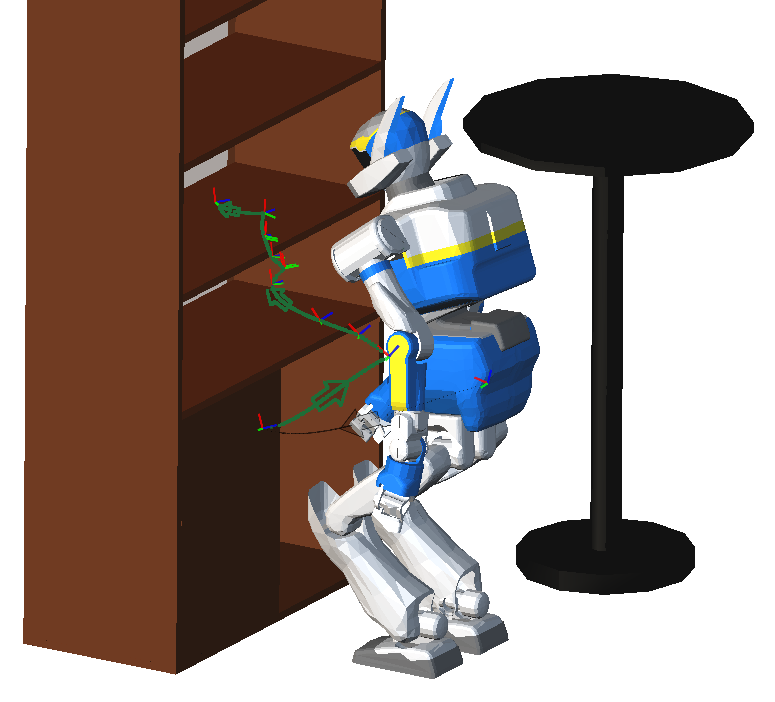
\includegraphics[width=0.8\linewidth]
                {src/chap3-optimal-motion-planning/figure/shelves-path.png}
\caption{Path found by the path planner in a shelves environment.}
\label{path}
\end{figure}

We use the constrained planner in \cite{dali09}, which is
implemented with the motion planning library KineoWorks\texttrademark
\cite{Laumond2006}. This planner allows generating a collision-free
path, while guaranteeing that the solution path lies on a manifold of
the configuration space. We want to generate for HRP-2 a
collision-free path that guarantees its quasi-static balance when it
is standing on both feet. We then define the manifold $\manifold$
with the following stack of equality constraints:

\begin{enumerate}
  \item Right foot has a fixed 6D transformation,
  \item Left foot has a fixed 6D transformation,
  \item Center of mass vertical projection lies in the center of the
    support polygon.
\end{enumerate}

Additionally, we would like to avoid choosing a single goal
configuration \config{g}, but instead define a goal task
\task{g}. This task can be defined by a sub-manifold
$\goalmanifold$\thinspace of the planning manifold $\manifold$. For a
simple object manipulation task, $\goalmanifold$\thinspace can be
defined as the intersection between $\manifold$\thinspace and the
manifold defined by the following stack of equality constraints:

\begin{enumerate}
  \item Gripper has the same 3D position as the object to grab.
  \item Gripper thumb is oriented vertically.
\end{enumerate}

Given a start configuration \config{s} a planning manifold $\manifold$
and a goal sub-manifold $\goalmanifold$, we first create a set of goal
configurations \config{g} by sampling a fixed number of configurations
in $\goalmanifold$, then we solve the path problem from \config{s} to
\config{g}. The constrained planner diffuses trees from \config{s} and
each configuration of \config{g}, and stops once at least one of the
goal configurations is in the same connected component as
\config{s}. A shortcut optimizer can then prune unnecessary waypoints
and smooth the solution path. Figure \ref{path} shows an example where
HRP-2 has to grab an object on the lower shelf and place it on the
upper shelf.

\section{(Self-)Collision Avoidance Constraints}
\label{distance-constraints}
In path planning, Boolean collision queries are used to validate or
invalidate configurations and hence the whole path. This is not enough
in optimal control, especially for gradient-based solvers where
constraint must be $C^1$. Furthermore we need to return negative
values of the distance in case of collision to provide the solver the
means to get out of collision.

We choose to use bounding capsules, like in
\cite{Kanoun2011}. Capsules are sphere swept segments; the
inter-capsule distance can be simply found by computing the distance
between the capsule axes, then subtracting their radii. Similarly, we
can compute the distance between a capsule and a polyhedron by
computing the distance between the capsule axis and the polyhedron,
then subtracting the radius. The returned distance can then become
negative in case of collision.

\subsection{Computing minimum bounding capsules}
In \cite{Kanoun2011}, bounding capsules parameters, i.e. the 2
endpoints $\mathbf{e_1}, \mathbf{e_2}$ and the radius $r$, were set by
hand to obtain the best fitting capsules around the body
geometries. We propose here to automatically find these parameters by
solving, offline and once for each body of the robot, the following
optimization problem:

\begin{equation}
  \min_{\mathbf{e_1}, \mathbf{e_2}, r} \ \ 
  \|\mathbf{e_2} - \mathbf{e_1}\| \pi r^2 + \frac{4}{3}\pi r^3
  \label{capsule-objective}
\end{equation}
\ \ \ subject to:
\begin{equation}
  \begin{array}{rcll}
    r - d(\mathbf{p},\mathbf{e_1e_2}) & \ge & 0\mbox{, for all }
    \mathbf{p} \in \mathcal{P}
    \label{capsule-constraint}
  \end{array}
\end{equation} 
where $d(\mathbf{p},\mathbf{e_1e_2})$ is the distance of $\mathbf{p}$
to line segment $\mathbf{e_1e_2}$.  Equations \ref{capsule-objective}
and \ref{capsule-constraint} mean we want to find the minimum-volume
capsule while ensuring all points $p$ of the underlying polyhedron
$\mathcal{P}$ lie inside the capsule. HRP-2 has 41 bodies, each body
polyhedron containing about 1000 points. We solve all 41 optimization
problems with RobOptim \cite{roboptim, moulard2012optimisation} and
the IPOPT solver \cite{Biegler2009} in less than 5s. Figure
\ref{hrp2-capsule} shows the best fitting bounding capsules
superimposed on the robot geometries.

Add figure 2 capsules with distance.

FIXME: Add figure with romeo, kuka, hrp2.

Add computation times for poly to capsule, vs poly to convex hull to
capsule.

%%  & number of bodies & mean number of vertices per body & computation time without convex hull (s) & computation time with convex hull (s)
%% hrp2 & 41 & ? & 46.8 & 7.50
%% romeo & 46 & ? & 410 & 27.6

Add figure poly, convex hull, capsule (superimposed?)

\begin{figure}
  \centering
  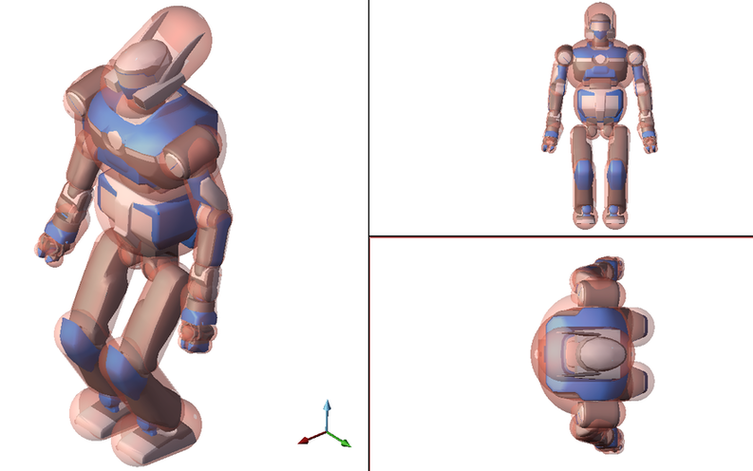
\includegraphics[width=0.9\linewidth]
                  {src/chap3-optimal-motion-planning/figure/hrp2-capsule-transparent.png}
  \caption{Best fitting capsules for HRP-2}
  \label{hrp2-capsule}
\end{figure}

\begin{figure}
  \centering
  \begin{subfigure}{0.48\columnwidth}
    \centering
    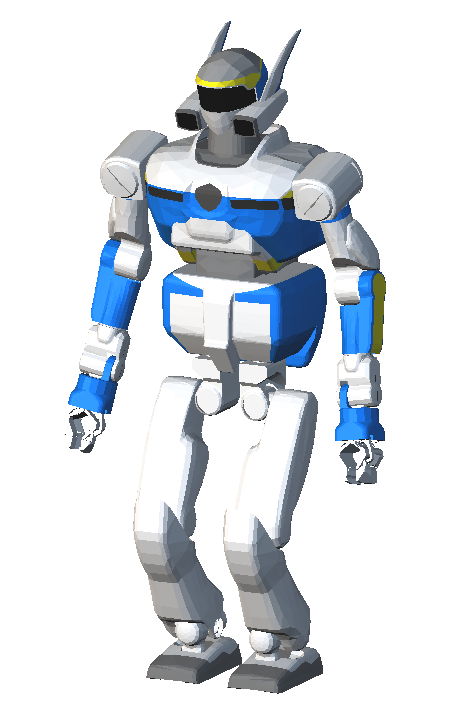
\includegraphics[width = \columnwidth]
                    {src/chap3-optimal-motion-planning/figure/hrp2-full-mesh.png}
    \caption{Initial invalid path.}
    \label{simple-patha}
  \end{subfigure}
  \begin{subfigure}{0.48\columnwidth}
    \centering
    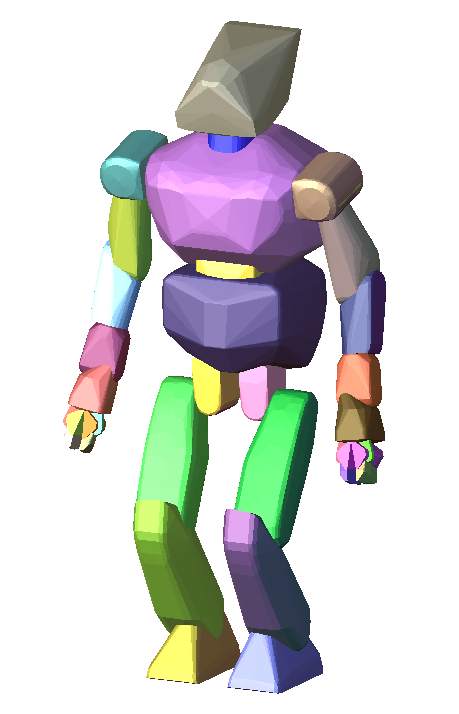
\includegraphics[width = \columnwidth]
                    {src/chap3-optimal-motion-planning/figure/hrp2-convex-hull.png}
    \caption{RRT path.}
    \label{simple-path-sola}
  \end{subfigure}
  \begin{subfigure}{0.48\columnwidth}
    \centering
    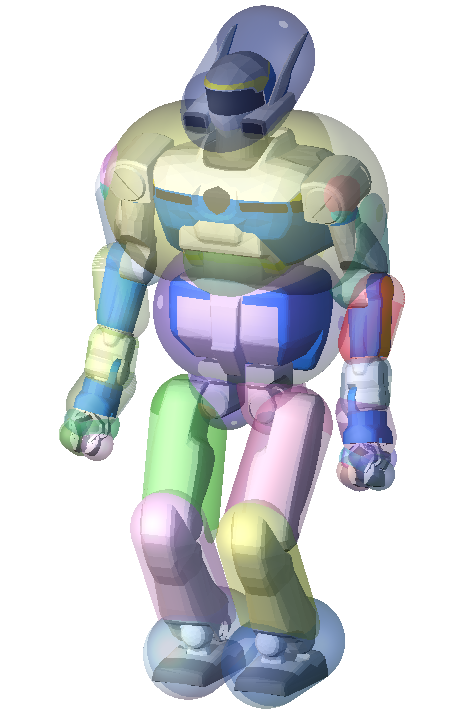
\includegraphics[width = \columnwidth]
                    {src/chap3-optimal-motion-planning/figure/hrp2-bounding-capsule.png}
    \caption{Shortcut path.}
    \label{simple-FIXMEa}
  \end{subfigure}
  \begin{subfigure}{0.48\columnwidth}
    \centering
    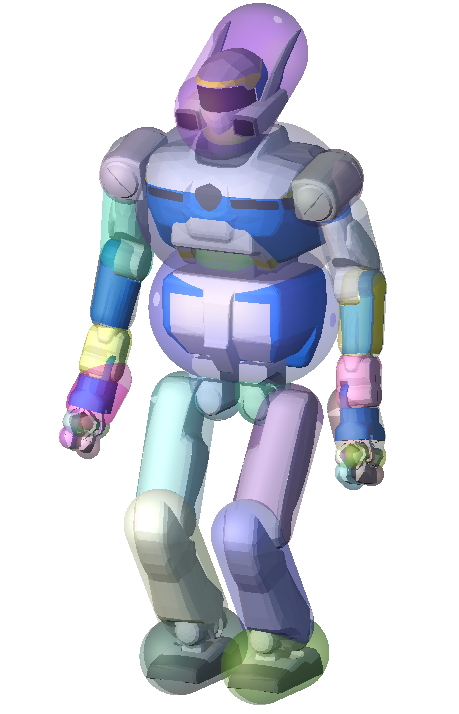
\includegraphics[width = \columnwidth]
                    {src/chap3-optimal-motion-planning/figure/hrp2-capsule.png}
    \caption{Shortcut path.}
    \label{simple-path-sol-shortcuta}
  \end{subfigure}
  \caption{Paths for the test case.}
\end{figure}

\begin{figure}
  \centering
  \begin{subfigure}{0.48\columnwidth}
    \centering
    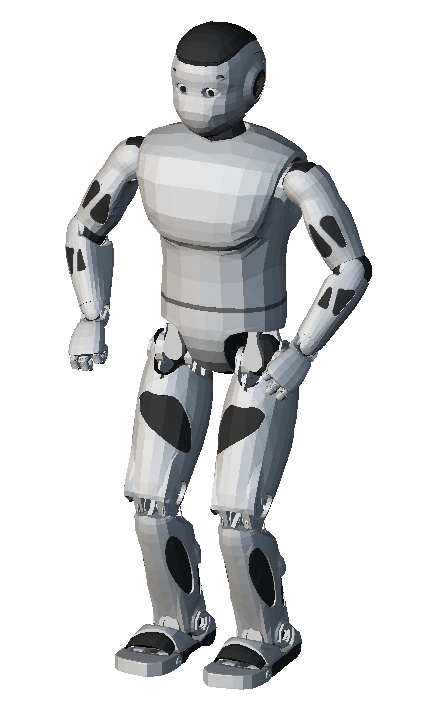
\includegraphics[width = \columnwidth]
                    {src/chap3-optimal-motion-planning/figure/romeo-full-mesh.png}
    \caption{Initial invalid path.}
    \label{simple-pathb}
  \end{subfigure}
  \begin{subfigure}{0.48\columnwidth}
    \centering
    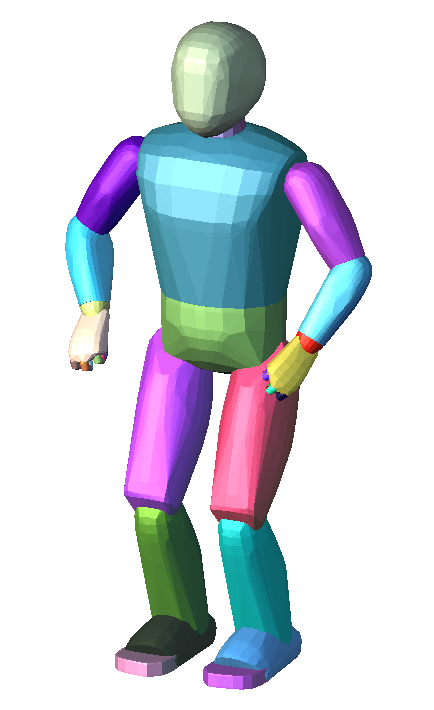
\includegraphics[width = \columnwidth]
                    {src/chap3-optimal-motion-planning/figure/romeo-convex-hull.png}
    \caption{RRT path.}
    \label{simple-path-solb}
  \end{subfigure}
  \begin{subfigure}{0.48\columnwidth}
    \centering
    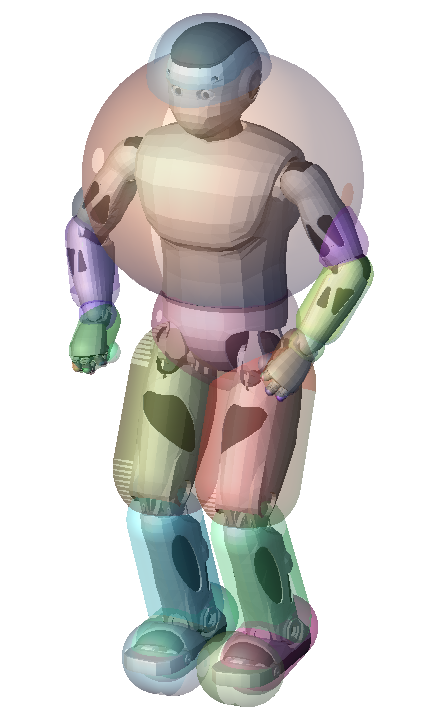
\includegraphics[width = \columnwidth]
                    {src/chap3-optimal-motion-planning/figure/romeo-bounding-capsule.png}
    \caption{Shortcut path.}
    \label{FIXMEb}
  \end{subfigure}
  \begin{subfigure}{0.48\columnwidth}
    \centering
    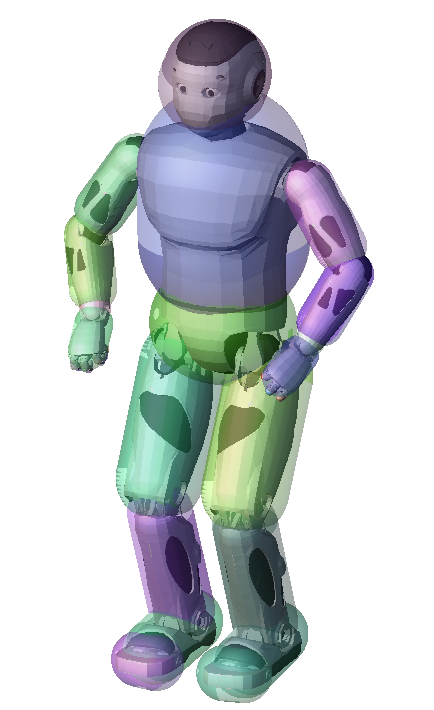
\includegraphics[width = \columnwidth]
                    {src/chap3-optimal-motion-planning/figure/romeo-capsule.png}
    \caption{Shortcut path.}
    \label{simple-path-sol-shortcutb}
  \end{subfigure}
  \caption{Paths for the test case.}
\end{figure}

\subsection{Distance computation}
As mentioned previously, for capsule-capsule distance pairs, we need
to compute the distance between the two capsule axes then subtract the
radii to obtain the real distance. We rely on the Wild Magic geometric
library \cite{schneider2003geometric, wildmagic} to compute this
distance in an average time of 2 $\mu$s.

Concerning capsule-polyhedron pairs, we rely on an implementation of
OBB-Trees in the Kineo Collision Detection (KCD) library
\cite{Laumond2006} for an efficient computation. For the environment
in figure \ref{path}, the distance for one capsule-environment pair
takes about 500 $\mu$s to be computed, since the environment is
assumed to be perfectly modeled by polyhedron meshes.

\subsection{Selection of pairs of bodies for distance computation}
If we take into account all capsule-capsule pairs of the robot, we end
up with $\frac{n(n - 1)}{2}$ possible pairs, with $n$ the number of
bodies. This means that for a robot like HRP-2, we can have up to 820
pairs and it can be very costly to evaluate the distance for all of
them. Luckily, some bodies are either always colliding because they
are adjacent in the kinematic tree, or never colliding due to the
joint limits; the pairs corresponding to those bodies can be safely
pruned. We use the tool described in \cite{planning-environment},
which relies on finely exploring the configuration space and keeping
track of colliding bodies, to save 510 useful pairs. Furthermore,
since we are in the particular case of double-support motion, we can
be sure that most of the leg bodies cannot collide with each other due
to the additional kinematic constraints. We finally end up with 327
capsule-capsule pairs that must be all evaluated to guarantee
self-collision avoidance. Similarly, we can prune some of the 41
capsule-environment pairs that do not need to be checked due to the
particular kinematic structure of the HRP-2. For instance, if both
waist and chest are not in collision with the environment, we can be
sure that it will be the same for the intermediate body linking
them. We thus keep 23 capsule-environment pairs.

\section{Description of Optimal Motion Planning Framework}
\label{framework}

Now that we have properly set distance pairs, we can establish a
complete formulation of the optimal control problem for the second
stage of our optimal motion planning framework.

\subsection{Optimal Control Problem Formulation}

\subsubsection{Objective function}

We choose to minimize, for a fixed duration, the integral over time of
the sum of square jerks, as this criterion leads to smooth and natural
trajectories.

The objective function can then be written as:
\begin{equation}
  J = \int_{0}^{T}\mathbf{\dddot{q}}(t)^T\mathbf{\dddot{q}}(t) dt
  \label{objective-function}
\end{equation}

and we define the state and control variables to be:
\begin{equation}
  \begin{array}{rcl}
  \mathbf{x}(t) & = & [\mathbf{q}(t), \mathbf{\dot{q}}(t), \mathbf{\ddot{q}}(t)]^T \\
  \mathbf{u}(t) & = & [\mathbf{\dddot{q}}(t)]^T
  \end{array}
  \label{variables}
\end{equation}

\subsubsection{Equality and inequality constraints}

\paragraph{Joint constraints}
% and mechanical structure
Each actuated joint is subject to physical limitations of its
underlying actuator. Box constraints on angular, speed and torque
limits are then added as:

\begin{equation}
  \begin{array}{rcccl}
    \mathbf{q_{min}} & \le & \mathbf{q} & \le & \mathbf{q_{max}} \\
    \mathbf{\dot{q}_{min}} & \le & \mathbf{\dot{q}} & \le & \mathbf{\dot{q}_{max}} \\
    \mathbf{\tau_{min}} & \le & \mathbf{\tau} & \le & \mathbf{\tau_{max}}
  \end{array}
  \label{joint-constraints}
\end{equation}

\paragraph{Dynamic balance}
The robot is submitted in our case to multiple coplanar contact
reaction forces from the ground. We can then express the dynamic
balance constraint using the Zero-Moment Point (ZMP)
\cite{Vukobratovic2004zero}, which has to remain inside the robot
support polygon defined by its feet.

These constraints can be written as for any $t\in[0,T]$:
\begin{equation}
  \begin{array}{rcl}
    \mathbf{p_{lf}}(\mathbf{q}(t)) & = & \mathbf{p_{lf}}(\mathbf{q}(0)) \\
    \mathbf{p_{rf}}(\mathbf{q}(t)) & = & \mathbf{p_{rf}}(\mathbf{q}(0)) \\
    \mathbf{zmp} (\mathbf{q}(t), \mathbf{\dot{q}}(t), \mathbf{\ddot{q}}(t)) & \in & \mathcal{P}_{sup},
  \end{array}
  \label{dynamic-constraints}
\end{equation}

where $\mathbf{p_{lf}}$, $\mathbf{p_{rf}}$ are respectively the 6D
positions of the left and right feet, $\mathbf{zmp}$ and
$\mathcal{P}_{sup}$ are the ZMP coordinates and the support polygon
respectively.

\paragraph{Collision avoidance constraints}
We use the capsule-capsule and capsule-environment pairs defined in
\ref{distance-constraints}. Given a configuration \config{} of the
robot, we check that distances for pairs of bodies and pairs of body
and obstacle are positive to ensure (self-)collision avoidance. We
first tried to add one constraint per pair, which added up to $(327 +
23)*n_{ms}$ constraints, where $n_{ms}$ is the number of multiple
shooting nodes in \textsc{MUSCOD-II}. This led to poor performance as
the solver systematically went beyond the threshold number of
iterations. We hence propose to group all pairs for each single body
and define as an inequality constraint, the minimum distance of the
body to other bodies and to the obstacles being positive.

\subsection{Considerations for the Solver}
\label{initial-guess}
With a complete formulation of the optimal control problem, the solver
starts from an initial value of $\mathbf{q}(t)$ and $\mathbf{u}(t)$
and converges iteratively towards the locally optimal solution. It is
then obvious that the initial guess plays an important role in the
successful determination of the final solution and the convergence
speed.

The constrained path planner generates a collision-free path where the
kinematic constraints are enforced, but we still need to apply a time
parametrization before feeding it to the optimization solver. We want
to minimize the sum of square jerks; \cite{Flash1985} shows that an
unconstrained minimum-jerk trajectory is a polynomial of degree 5
which can be explicitly computed if the initial and final states are
known. We choose then to place minimum-jerk trajectories between each
pair of path waypoints, assuming they start and end at zero velocity
and acceleration. This ensures that the configuration $\mathbf{q}(t)$
follows exactly the solution path and that collision avoidance
constraints are not violated. The optimization solver will then
reshape this initial guess while enforcing all constraints, leading to
a smooth motion without intermediate stops.

In order to solve a finite-dimension optimal problem, we need to
discretize both controls and constraints. We thus define the control
u(t) as a continuous piecewise linear function over 20 sub-intervals
of the whole trajectory duration.

\section{Results}
\label{results}

\begin{figure}
  \centering
  \begin{subfigure}{0.32\columnwidth}
    \centering
    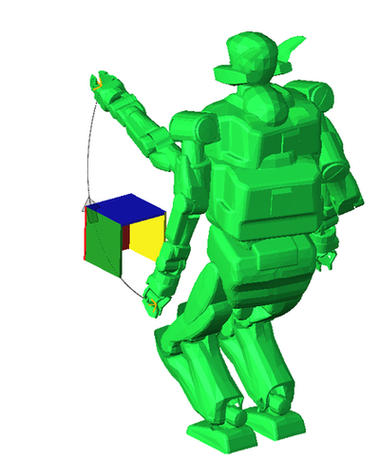
\includegraphics[width = \columnwidth]
                    {src/chap3-optimal-motion-planning/figure/simple-path.png}
    \caption{Initial invalid path.}
    \label{simple-path}
  \end{subfigure}
  \begin{subfigure}{0.32\columnwidth}
    \centering
    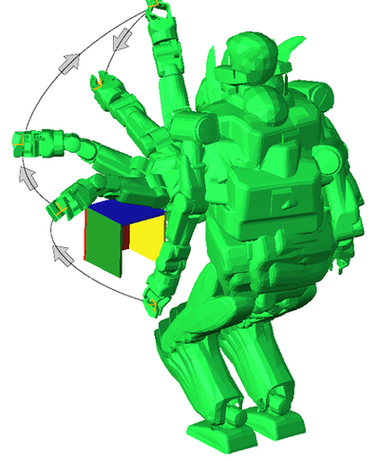
\includegraphics[width = \columnwidth]
                    {src/chap3-optimal-motion-planning/figure/simple-path-sol.png}
    \caption{RRT path.}
    \label{simple-path-sol}
  \end{subfigure}
  \begin{subfigure}{0.32\columnwidth}
    \centering
    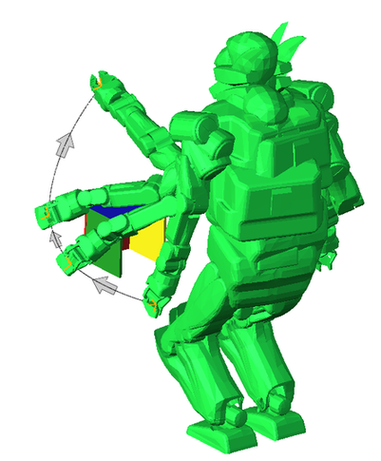
\includegraphics[width = \columnwidth]
                    {src/chap3-optimal-motion-planning/figure/simple-path-sol-shortcut.png}
    \caption{Shortcut path.}
    \label{simple-path-sol-shortcut}
  \end{subfigure}
  \caption{Paths for the test case.}
\end{figure}

We demonstrate the effectiveness of our optimal motion planning
framework by first using it in a a simple test case example, then
applying it to generate feasible motions on the robot HRP-2. All tests
were run on a computer with a 2.53 GHz
Intel\textsuperscript{\textregistered} Core\texttrademark2 Duo
processor.

\subsection{Test Case}
\label{test-case}
Figure \ref{simple-path} shows the motion planning problem to be
solved: HRP-2 starts from its rest position and moves to a goal
configuration by raising its left arm. A concave object is placed such
that the left hand is at one point enclosed in it if the initial path
connecting the start to goal configuration is executed. This is a
typical example of a problem with a local minimum defined by the
environment, where a real-time control approach in task-space might
fail. Figure \ref{simple-path-sol} shows a possible solution path
found with constrained RRT. This path can be shortened with a shortcut
optimizer, as in figure \ref{simple-path-sol-shortcut}.

To showcase the usefulness of our approach, we try to solve the
optimal control problem defined in Section \ref{framework} starting
from the different paths, and put all results in Table
\ref{table}. When starting with the initial path from figure
\ref{simple-path}, the solver failed to achieve a single
iteration. This can be explained by the fact that in the middle of
this path, the robot left hand is enclosed inside the obstacle and
some distance constraints are violated; the solver fails to determine
a clear direction which would remove this violation due to the
geometric local minimum. Since the constrained RRT avoids it and
generates a collision-free path, the solver behaves correctly when
starting with the path in \ref{simple-path-sol}, but the maximum
number of iterations is reached before reaching convergence. It is
achieved when starting with the shortcut path in
\ref{simple-path-sol-shortcut}. Note that about 70\% of the
optimization time is spent in evaluating the distance constraints and
their gradients; this significant overhead can be explained by the
fact that \textsc{MUSCOD-II} relies on internal numerical
differentiation to compute Jacobians. Relying on analytical gradient
expressions would thus accelerate the optimization process. Regarding
the distance constraints enforcement, figure
\ref{simple-distance-constraints} shows the evaluation of the left arm
distances: due to the constraints time discretization, one constraint
is violated during less than 100ms. This violation does not however
exceed 4mm, and this is considered as acceptable as all distance
constraints are computed with bounding capsule geometries which
already define conservative volumes around the exact geometries.

\begin{table}
  \renewcommand{\arraystretch}{1.3}
  \caption{Test Case Computation Times}
  \label{table}
  \centering
  \begin{tabular}{|c||c|c|c|}
    \hline
    Initial guess & Initial path & RRT path & Shortcut path \\
    \hline
    Planning time (s) & -- & 5 & 5 \\
    \hline
    Shortcut time (s) & -- & -- & 4 \\
    \hline
    Optimization status & ERROR & MAX\_ITER & OK \\
    \hline
    SQP iterations & -- & 200 & 70 \\
    \hline
    Optimization time (s) & -- & 3068 & 1186 \\
    \hline
    Constraints evaluation time (s) & -- & 2176 & 847 \\
    \hline
  \end{tabular}
\end{table}

FIXME: remove figure and plot from data instead? or use matplotlib to
make nicer plot.

\begin{figure}
  \centering
  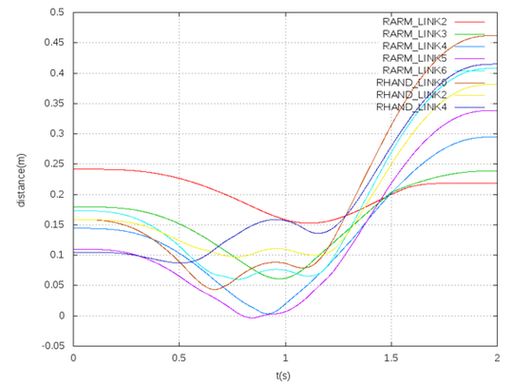
\includegraphics[width=0.8\linewidth]
                  {src/chap3-optimal-motion-planning/figure/distance-constraints.png}
  \caption{Plots of left arm body distance constraints.}
  \label{simple-distance-constraints}
\end{figure}

\subsection{Fast Trajectory Generation on HRP-2}

We also use our approach to generate fast optimal collision-free
trajectories and execute them on the humanoid robot HRP-2. In the
first scenario, HRP-2 executes a kind of martial art figure where it
crosses its arms rapidly while bending its knees, changes the arms
configuration, then moves back to a rest posture. The motion must be
executed while ensuring the arms do not collide with each other, and
the robot does not fall. This is quite a difficult task as the 3
trajectories durations are fixed to 1, 2, and 2 seconds
respectively. Particularly, the second motion where one arm goes from
being behind the other arm to being ahead of it proved to be
impossible to generate without a prior planning phase as proposed in
out approach.

In the second scenario, we add a complex environment that contains
shelves with different levels; HRP-2 first bends its knees to grab a
ball located deep on the lower shelf, then moves it to an upper shelf
to release it between two other objects. The trajectories last
respectively 2 and 5 seconds. Here, both collision and self-collision
constraints need to be enforced in order to obtain a valid
trajectory. Again, the ball transfer motion cannot be generated using
an optimal control solver and a simple initial guess; a prior planning
phase is needed to find a collision-free transfer path.

We successfully apply our framework to generate feasible motions for
both scenarios as seen in figures \ref{self-collision} and
\ref{shelves}. Computation times are shown in Tables
\ref{table-martial-art} and \ref{table-shelves}. Videos of both
scenarios are available in the attached file.

\begin{figure}
  \centering
  \begin{subfigure}{0.19\columnwidth}
    \centering
    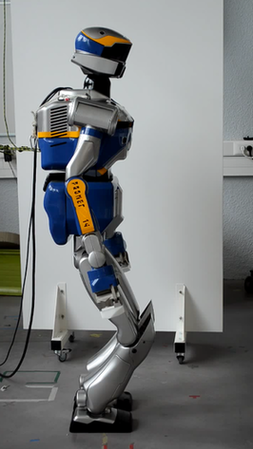
\includegraphics[width = \columnwidth]
                    {src/chap3-optimal-motion-planning/figure/self-collision-1.png}
    \label{self-collision-1}
  \end{subfigure}
  \begin{subfigure}{0.19\columnwidth}
    \centering
    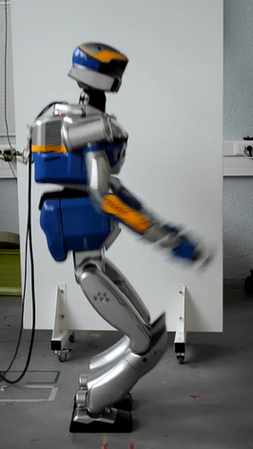
\includegraphics[width = \columnwidth]
                    {src/chap3-optimal-motion-planning/figure/self-collision-2.png}
    \label{self-collision-2}
  \end{subfigure}
  \begin{subfigure}{0.19\columnwidth}
    \centering
    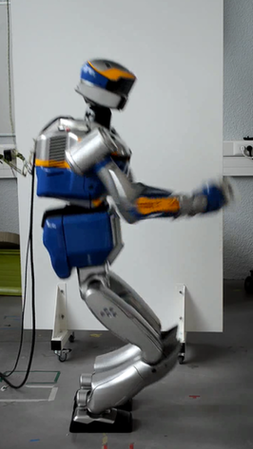
\includegraphics[width = \columnwidth]
                    {src/chap3-optimal-motion-planning/figure/self-collision-3.png}
    \label{self-collision-3}
  \end{subfigure}
  \begin{subfigure}{0.19\columnwidth}
    \centering
    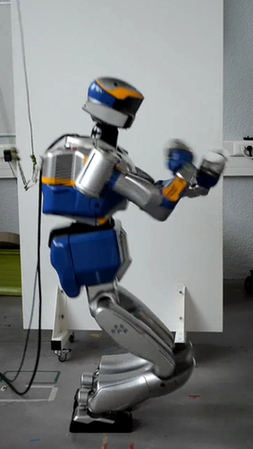
\includegraphics[width = \columnwidth]
                    {src/chap3-optimal-motion-planning/figure/self-collision-4.png}
    \label{self-collision-4}
  \end{subfigure}
  \begin{subfigure}{0.19\columnwidth}
    \centering
    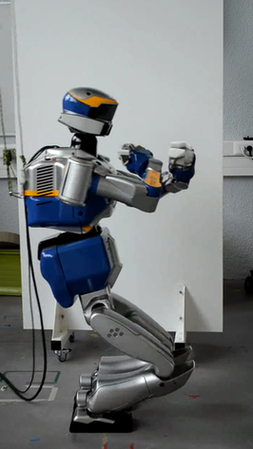
\includegraphics[width = \columnwidth]
                    {src/chap3-optimal-motion-planning/figure/self-collision-5.png}
    \label{self-collision-5}
  \end{subfigure}
  \begin{subfigure}{0.19\columnwidth}
    \centering
    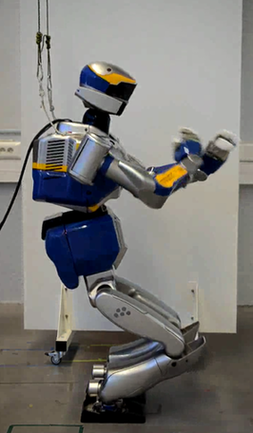
\includegraphics[width = \columnwidth]
                    {src/chap3-optimal-motion-planning/figure/self-collision-6.png}
    \label{self-collision-6}
  \end{subfigure}
  \begin{subfigure}{0.19\columnwidth}
    \centering
    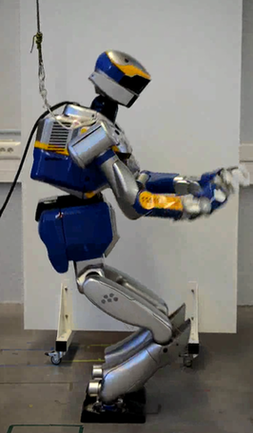
\includegraphics[width = \columnwidth]
                    {src/chap3-optimal-motion-planning/figure/self-collision-7.png}
    \label{self-collision-7}
  \end{subfigure}
  \begin{subfigure}{0.19\columnwidth}
    \centering
    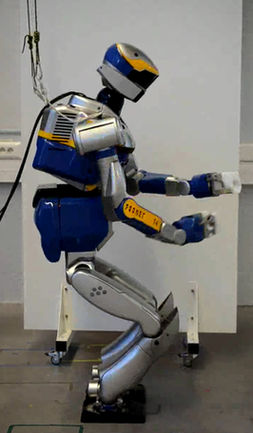
\includegraphics[width = \columnwidth]
                    {src/chap3-optimal-motion-planning/figure/self-collision-8.png}
    \label{self-collision-8}
  \end{subfigure}
  \begin{subfigure}{0.19\columnwidth}
    \centering
    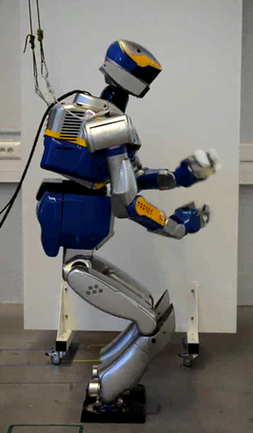
\includegraphics[width = \columnwidth]
                    {src/chap3-optimal-motion-planning/figure/self-collision-9.png}
    \label{self-collision-9}
  \end{subfigure}
  \begin{subfigure}{0.19\columnwidth}
    \centering
    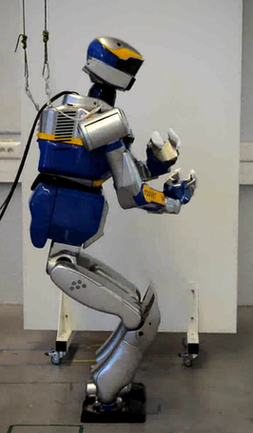
\includegraphics[width = \columnwidth]
                    {src/chap3-optimal-motion-planning/figure/self-collision-10.png}
    \label{self-collision-10}
  \end{subfigure}
  \caption{HRP-2 does a quick martial arts motion while avoiding
    self-collision.}
  \label{self-collision}
\end{figure}

\begin{figure}
  \centering
  \begin{subfigure}{0.19\columnwidth}
    \centering
    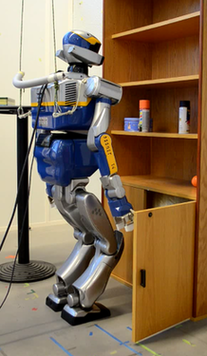
\includegraphics[width = \columnwidth]
                    {src/chap3-optimal-motion-planning/figure/shelves-1.png}
    \label{shelves-1}
  \end{subfigure}
  \begin{subfigure}{0.19\columnwidth}
    \centering
    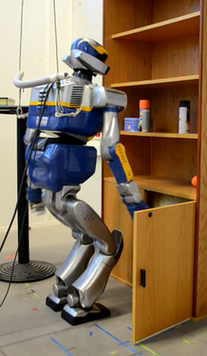
\includegraphics[width = \columnwidth]
                    {src/chap3-optimal-motion-planning/figure/shelves-2.png}
    \label{shelves-2}
  \end{subfigure}
  \begin{subfigure}{0.19\columnwidth}
    \centering
    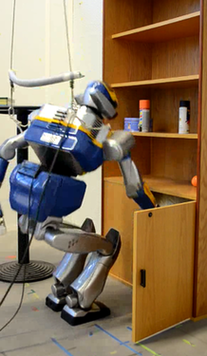
\includegraphics[width = \columnwidth]
                    {src/chap3-optimal-motion-planning/figure/shelves-3.png}
    \label{shelves-3}
  \end{subfigure}
  \begin{subfigure}{0.19\columnwidth}
    \centering
    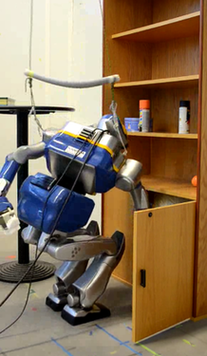
\includegraphics[width = \columnwidth]
                    {src/chap3-optimal-motion-planning/figure/shelves-4.png}
    \label{shelves-4}
  \end{subfigure}
  \begin{subfigure}{0.19\columnwidth}
    \centering
    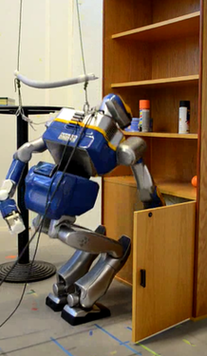
\includegraphics[width = \columnwidth]
                    {src/chap3-optimal-motion-planning/figure/shelves-5.png}
    \label{shelves-5}
  \end{subfigure}
  \begin{subfigure}{0.19\columnwidth}
    \centering
    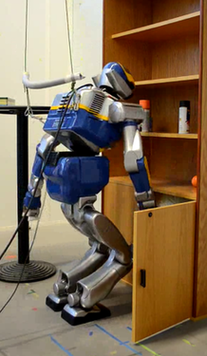
\includegraphics[width = \columnwidth]
                    {src/chap3-optimal-motion-planning/figure/shelves-6.png}
    \label{shelves-6}
  \end{subfigure}
  \begin{subfigure}{0.19\columnwidth}
    \centering
    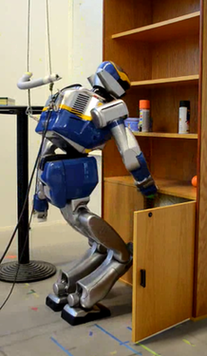
\includegraphics[width = \columnwidth]
                    {src/chap3-optimal-motion-planning/figure/shelves-7.png}
    \label{shelves-7}
  \end{subfigure}
  \begin{subfigure}{0.19\columnwidth}
    \centering
    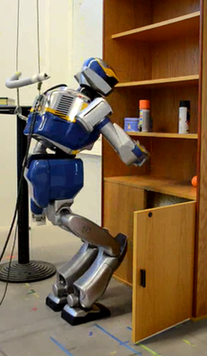
\includegraphics[width = \columnwidth]
                    {src/chap3-optimal-motion-planning/figure/shelves-8.png}
    \label{shelves-8}
  \end{subfigure}
  \begin{subfigure}{0.19\columnwidth}
    \centering
    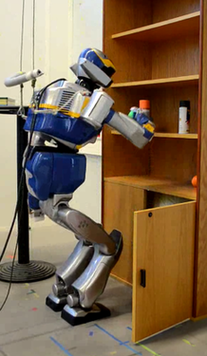
\includegraphics[width = \columnwidth]
                    {src/chap3-optimal-motion-planning/figure/shelves-9.png}
    \label{shelves-9}
  \end{subfigure}
  \begin{subfigure}{0.19\columnwidth}
    \centering
    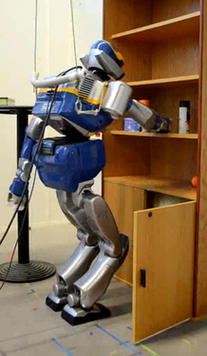
\includegraphics[width = \columnwidth]
                    {src/chap3-optimal-motion-planning/figure/shelves-10.png}
    \label{shelves-10}
  \end{subfigure}
  \caption{HRP-2 bends down quickly to grab a ball in the lower
    shelf and transfers it to the upper shelf.}
  \label{shelves}
\end{figure}

\begin{table}
  \renewcommand{\arraystretch}{1.3}
  \caption{Computation Times for Martial Arts Scenario}
  \label{table-martial-art}
  \centering
  \begin{tabular}{|c||c|c|c|}
    \hline
    Phase & 1 & 2 & 3 \\
    \hline
    Planning time (s) & 4 & 13 & 2 \\
    \hline
    Shortcut time (s) & 4 & 6 & 1 \\
    \hline
    SQP iterations & 32 & 73 & 25 \\
    \hline
    Optimization time (s) & 346 & 1130 & 278 \\
    \hline
    Constraints evaluation time (s) & 124 & 356 & 83 \\
    \hline
  \end{tabular}
\end{table}

\begin{table}
  \renewcommand{\arraystretch}{1.3}
  \caption{Computation Times for the Shelves Scenario}
  \label{table-shelves}
  \centering
  \begin{tabular}{|c||c|c|}
    \hline
    Phase & 1 & 2 \\
    \hline
    Planning time (s) & 13 & 38 \\
    \hline
    Shortcut time (s) & 6 & 23 \\
    \hline
    SQP iterations & 74 & 80 \\
    \hline
    Optimization time (s) & 1745 & 5020 \\
    \hline
    Constraints evaluation time (s) & 1396 & 2640 \\
    \hline
  \end{tabular}
\end{table}

\subsection{Discussion}
\label{discussion}

In subsection \ref{test-case}, we demonstrate in a simple example the
influence of the initial guess of the optimal control problem on the
solver success and performance. In fact, due to its probabilistic
completeness, the usage of the constrained planner in a first stage
guarantees that an initial collision-free and quasi-statically
feasible trajectory can be found. The optimization solver then can
reshape this trajectory in order to minimize the objective function
while enforce constraints such as joint limits and dynamic
balance. Note that with this method, locally optimal trajectories are
found; in order to find global optima, it might be interesting to plan
in \cspace\thinspace using RRT* instead of RRT in the first stage.

The trajectory duration is for the moment fixed. This means that if it
is not properly set, the optimization solver might fail as some
constraints such as velocity limits would never be enforced. If it is
included as a free variable in the optimal control problem, we will
have a guarantee of success for the second stage. The complete
framework would then always succeed in generating optimal
trajectories.

\section{Conclusion}
In this chapter we propose a novel approach to tackle optimal control
problems in cluttered environments. Our approach combines, in a
two-stage framework, a constrained path planning algorithm and an
optimal control problem solver. We generate optimal feasible
trajectories for the humanoid robot HRP-2 and successfully execute
them.

Our framework can benefit from improvements to increase its
usability. Future work will consider non-coplanar contacts, as well as
release the robot from its fixed support constraints in order to
accomplish optimal locomotion planning.

FIXME: add transition towards general conclusion.
